\section{Performance Evaluation}
\label{sec:performance}
To evaluate \textsc{Synopsis}, we used a real-world dataset to populate the distributed sketch. This includes dynamic scaling and an analysis of node stability as scaling operations take place, as well as query evaluation latencies for each query type. \\

\subsection{Dataset and Experimental Setup}
Our subject dataset was sourced from the NOAA North American Mesoscale (NAM) Forecast System \cite{noaa_nam}.  The NAM collects atmospheric data several times per day and includes features of interest such as surface temperature, visibility, relative humidity, snow, and precipitation. Each observation in the dataset also incorporates a relevant geographical location and time of creation. This information is used during the data ingest process to partition streams across available computing resources and preserve temporal ordering of events.

Our performance evaluation was carried out on a 75-node heterogeneous cluster consisting of 45 HP DL160 servers (Xeon E5620, 12 GB RAM) and 30 HP DL320e servers (Xeon E3-1220 V2, 8 GB RAM) running Fedora 23. \textsc{Synopsis} was executed under the OpenJDK Java runtime, version 1.8.0\_72. \\

\subsection{Dynamic Scaling}
\begin{figure}
    \centerline{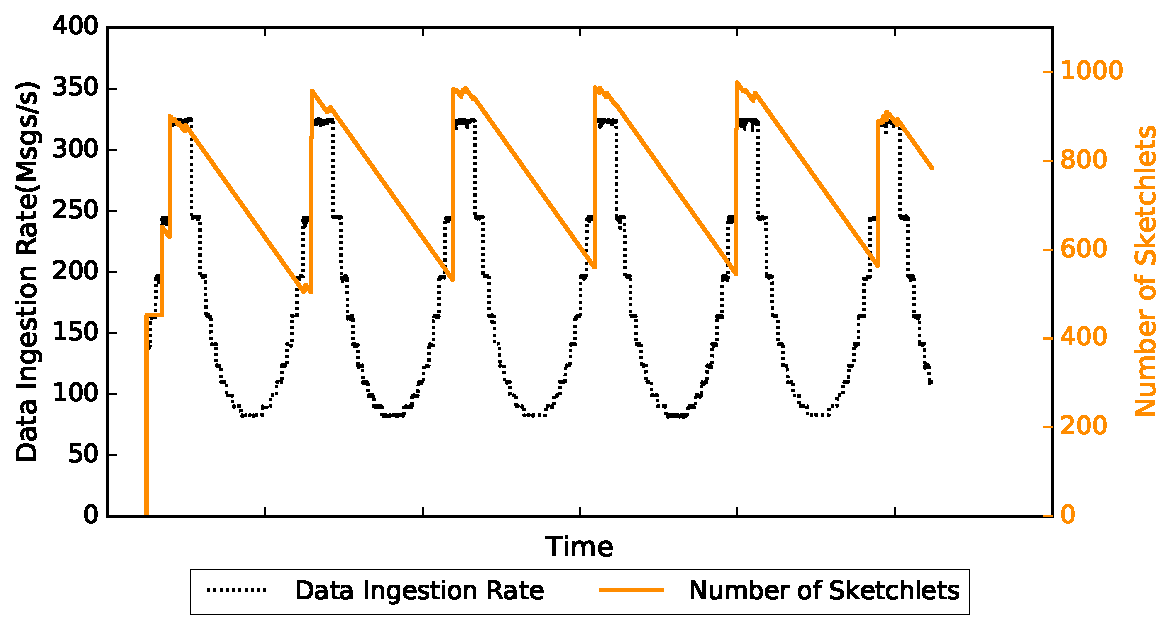
\includegraphics[width=3.5in]{figures/dyn-scaling.pdf}}
    \caption{The variation of number of sketchlets with the data ingestion rate.}
    \label{fig:dyn-scaling}
\end{figure}
We evaluated how \textsc{Synopsis} dynamically scales when the data ingestion rate is varied.
The data ingestion rate was varied over time such that the peak data ingestion rate is less than the highest possible throughput that will create a backlog at \textsc{Synopsis} nodes.
We used the number of sketchlets created in the system to quantify the scaling activities.
If the system scales out, more sketchlets will be created in child nodes after the targeted load migration.
We started with a single \textsc{Synopsis} node and allowed the system to dynamically scale.
As can be observed in Figure~\ref{fig:dyn-scaling}, the number of sketchlets varies with the ingestion rate.
Since we allow aggressive scale out, it shows a rapid scale out activity during high data ingestion rates whereas scaling in takes place gradually with one sub region (hence one sketch) at a time.
% scale out graph
\begin{figure*}
    \centerline{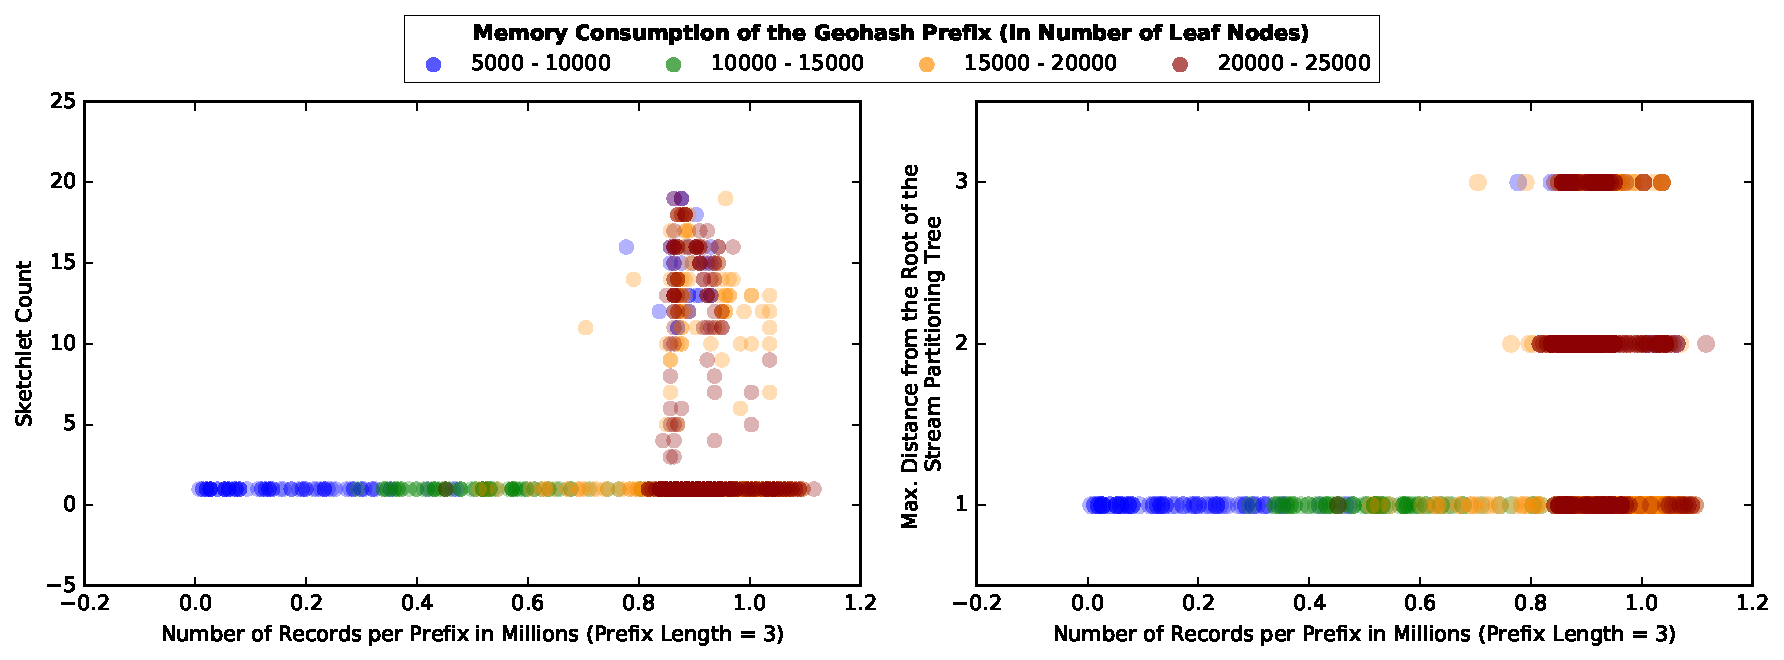
\includegraphics[width=\linewidth]{figures/scaleout_graph_analysis.pdf}}
    \caption{Analysis of a snapshot of stream processing graph during ingestion}
    \label{fig:scaleout-graph-analysis}
\end{figure*}

Figure~\ref{fig:scaleout-graph-analysis} visualizes a snapshot of the stream processing graph in runtime which validates our dynamic scaling implementation. 
This represents the state of the system after consuming the complete NOAA dataset for 2014 and the graph contained 48 sketchlets. 
It shows the distribution and size of the information maintained across \textsc{Synopsis} nodes for each geohash prefix of length 3 against the number of records processed for that particular prefix.
The space requirement is measured in terms of the number of leaf nodes in the corresponding sketchlets.
For the majority of the prefixes, the space requirement increases with the number of records processed for a particular prefix.
If the data for a particular prefix is distributed across multiple sketchlets, then it is more likely to be a prefix with a high number of records as shown in the first subplot.
In such cases, some of these sketchlets are created in multiple iterations of scaling out operations from their original nodes which results in a higher distance from the root in the prefix tree. This is depicted in the second sub figure of Figure~\ref{fig:scaleout-graph-analysis}.
A few prefixes with high number of records can be observed with a low memory consumption and are distributed across multiple sketchlets.
Their observations spans across a smaller range, hence requires less memory but they were chosen for scaling out operations due to their high message rates. 


\subsection{Stability at Individual Nodes}
The objective of this benchmark was to demonstrate how scaling out operations manage to maintain stability at each node under varying workload conditions.
The same setup as in previous micro benchmark was used, but the evaluation metrics captured are corresponding to an individual node instead of the entire system.
For this experiment, we have enabled only a single threshold-based rule (either backlog growth based or memory usage based) at a time to demonstrate its effectiveness.

We captured how backlog length and throughput at an individual node vary with the input rate when dynamic scaling is enabled.
The \textsc{Synopsis} node that was considered for the experiment immediately received data from stream ingesters, hence the input rate observed at the node closely resembled the varying data ingestion rate.
As shown in Figure~\ref{fig:stability-backlog}, scaling out helps a node to keep up with the variations in the workload which in turn causes the backlog to stay within a safe range.
It also demonstrates the infrequent rapid scaling out activities and the continuous gradual downscaling activities as explained in section~\ref{subsec:scaling-out}.

Figure~\ref{fig:stability-mem} demonstrates how memory consumption based threshold-based rules trigger scaling manures to maintain the system stability.
We have used a 0.45 of the total available memory for a JVM process as the upper threshold for triggering a scale out operation.
In certain occasions, it is required to perform multiple consecutive scaling out operations (interleaved with the cooling down periods) to bring the memory usage to the desired level due to the increased memory utilization caused by the data ingestion happening in the background.
% system stability
\begin{figure*}
    \begin{subfigure}{0.48\textwidth}
            \centering
            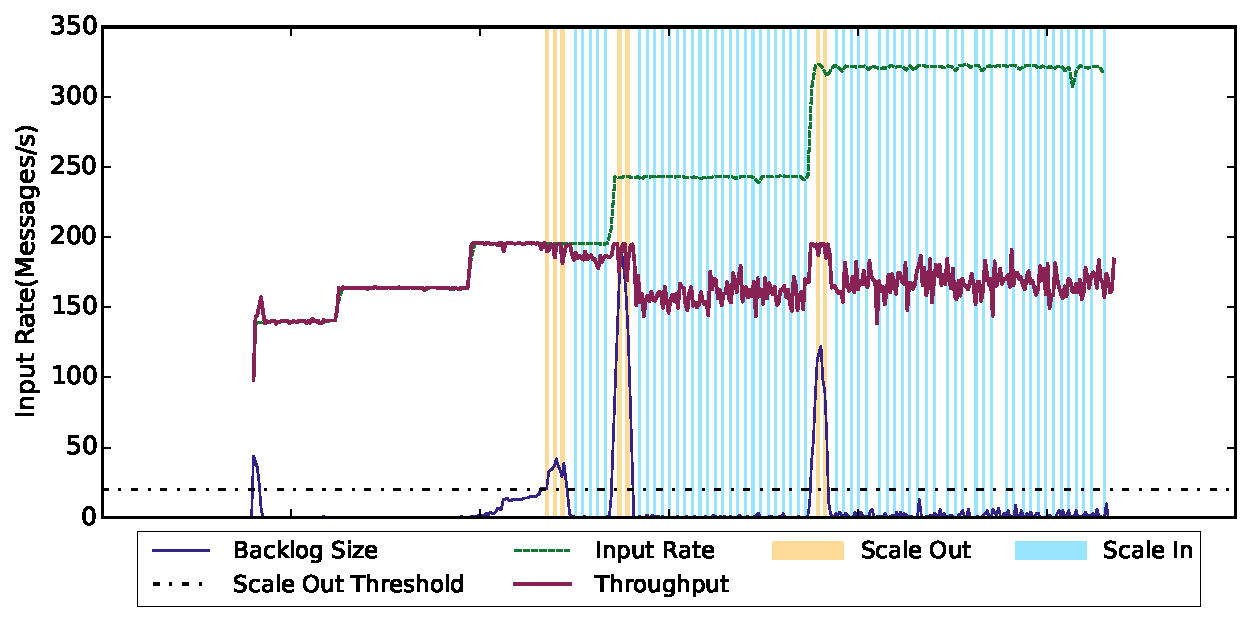
\includegraphics[scale=0.42]{figures/stability_partial.pdf}
            \caption{Dynamic scaling manures triggered by backlog growth based threshold rules}
            \label{fig:stability-backlog}
    \end{subfigure}
    \begin{subfigure}{0.48\textwidth}
            \centering
            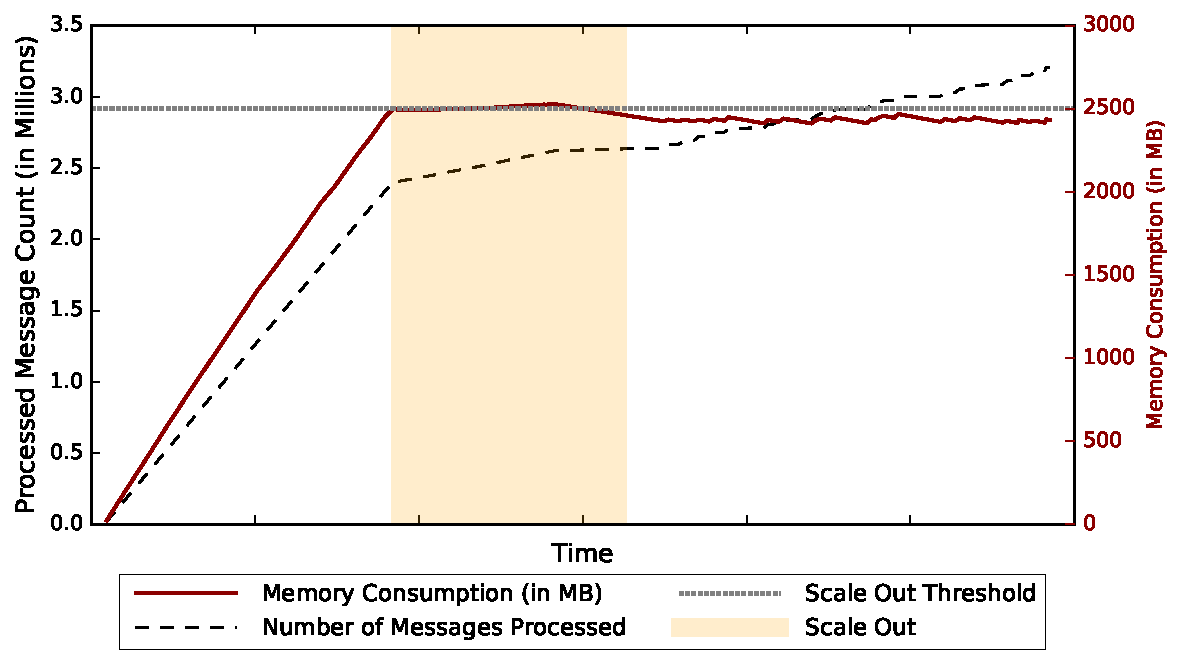
\includegraphics[scale=0.42]{figures//mem_stability.pdf} 
            \caption{Dynamic scaling manures triggered by memory usage based threshold rules}
            \label{fig:stability-mem}
    \end{subfigure}
    \caption{How scaling out enables maintaining stability at an individual \textsc{Synopsis} node based on backlog growth and memory usage}
    \label{fig:system-stability}
\end{figure*}


% system benchmark on mem. consumption
\begin{figure}
    \centerline{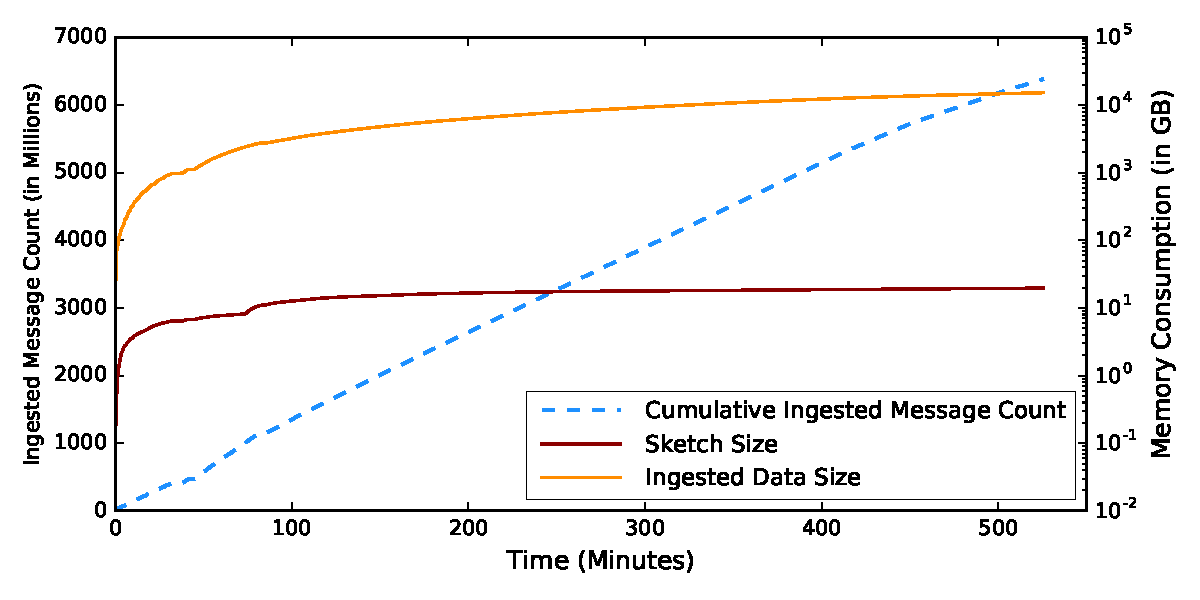
\includegraphics[width=\linewidth]{figures/ing-and-mem-usage.pdf}}
    \caption{Memory usage of the distributed sketch over time against the amount of ingested data}
    \label{fig:dist-sketch-mem-usage}
\end{figure}


\subsection{Sketch Query Evaluation}
To evaluate the performance of the sketch, we executed several representative query workloads across a variety of sketchlet sizes. These queries were separated into two groups: data structure lookups and graph lookups. Data structure lookups include density queries, set queries, and summary statistics for the entire sketch, while graph lookups involve targeted portions of the overall feature space. In general, queries that require a graph lookup consume more processing time, but are much more expressive; for instance, such a query could request summary statistics or feature relationships when the temperature is between 20 to 30 degrees, humidity is above 80\%, and the wind is blowing at 16 km/h, while a data structure lookup would be restricted to chronological parameters and select features of interest. Table~\ref{tbl:query-times} outlines the query times for both evaluation types. In general, data structure lookup operations require minimal processing. While graph lookups take longer to complete, it is worth noting that varying the geographical scope across sketchlet sizes from 5km to 800km did not result in a proportionate increase in processing time. Overall, the sketch is able to satisfy our goal of low-latency query evaluations for each query type. \\ \vspace{2.5em}

\begin{table}[h!]
    \renewcommand{\arraystretch}{1.4}
    \caption{Query evaluation times for each query type (averaged over 1000 iterations).}
    \label{tbl:query-times}
    \begin{center}
        \begin{tabular}{|l|c|c|}
            \hline
            \textbf{Query Type}      & \textbf{Eval. (ms)} & \textbf{Std. Dev.} \\
            \hline
            Density                  & 0.007                    & 0.005 \\
            \hline
            Set Cardinality          & 0.154                    & 0.088 \\
            \hline
            Set Frequency            & 0.036                    & 0.019 \\
            \hline
            Set Membership           & 0.015                    & 0.009 \\
            \hline
            Statistics               & 0.002                    & 0.001 \\
            \hline
            \hline
            Subgraph Stat. (5 km)    & 46.357                   & 1.287 \\
            \hline
            Relational (5 km)        & 40.510                   & 6.937 \\
            \hline
            Relational (25 km)       & 47.619                   & 6.355 \\
            \hline
            Relational (800 km)      & 53.620                   & 6.818 \\
            \hline
        \end{tabular}
    \end{center}
\end{table}
% distributed query evaluation
\begin{figure*}
    \centerline{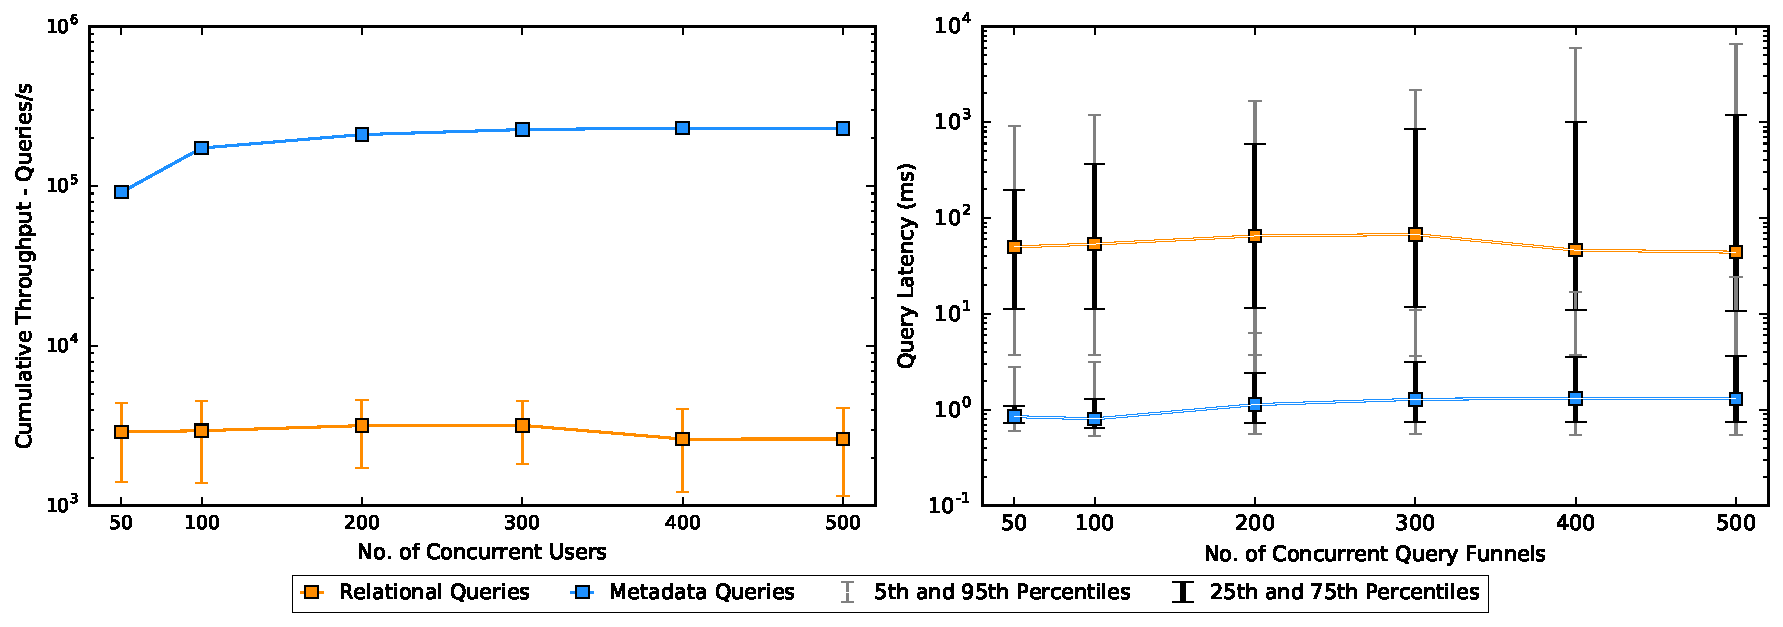
\includegraphics[width=\linewidth]{figures/query_benchmark_both.pdf}}
    \caption{Distributed Query Evaluation Performance}
    \label{fig:dist-query}
\end{figure*}


\begin{figure}
    \centerline{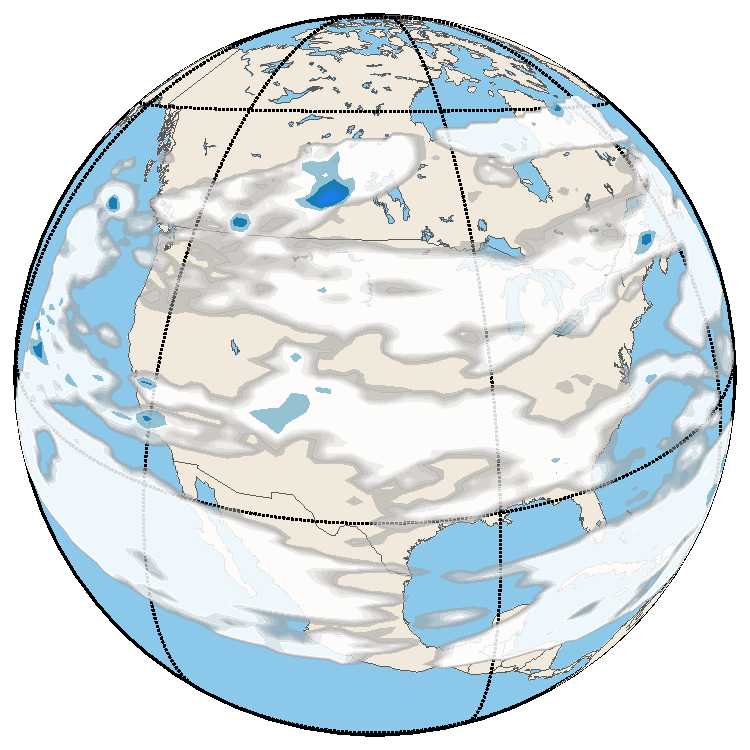
\includegraphics[width=\linewidth]{figures/globe.pdf}}
    \caption{Global contour visualization}
    \label{fig:global-contour}
\end{figure}

\begin{figure}
    \centerline{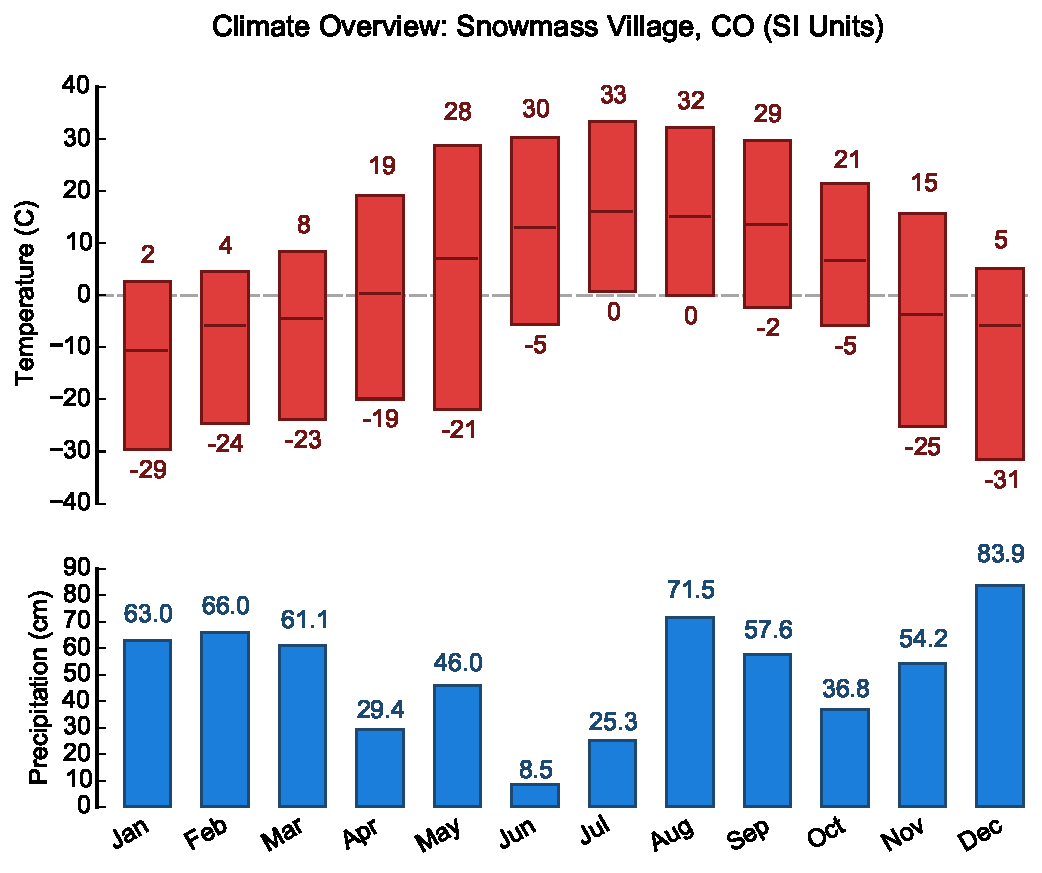
\includegraphics[width=\linewidth]{figures/climate-snowmass.pdf}}
    \caption{Climate chart visualization}
    \label{fig:climate}
\end{figure}

